\documentclass[12pt,a4paper]{article}
\usepackage[vietnamese]{babel}
\usepackage{fontspec}
\usepackage{indentfirst}
\usepackage{geometry}
\usepackage{graphicx}
\usepackage{float}
\usepackage[normalem]{ulem}
\usepackage{soul}
\usepackage{booktabs}
\usepackage{array}
\usepackage{longtable}
\usepackage{xurl}
\usepackage{hyperref}
\usepackage{fancyhdr}
\usepackage{pgfplots}
\usetikzlibrary{positioning,arrows.meta,shapes.geometric,shadows}
\pgfplotsset{compat=1.18}
\geometry{margin=1in}
\setmainfont{Times New Roman}
\setsansfont{Arial}
\setmonofont{Courier New}
\setlength{\parindent}{1.25em}
\setlength{\parskip}{0.35em}
\AtBeginDocument{\fontsize{13pt}{16pt}\selectfont}
\hypersetup{
  colorlinks=true,
  linkcolor=black,
  urlcolor=blue!55!black
}
\urlstyle{same}
\pagestyle{fancy}
\fancyhf{}
\rfoot{\thepage}
\renewcommand{\headrulewidth}{0pt}

\begin{document}

\begin{titlepage}
\centering
\vspace*{1cm}
{\bfseries\Large ĐẠI HỌC QUỐC GIA THÀNH PHỐ HỒ CHÍ MINH\par}
\vspace{0.5cm}
{\bfseries\Large TRƯỜNG ĐẠI HỌC CÔNG NGHỆ THÔNG TIN\par}
\vspace{0.5cm}
{\bfseries Trung tâm Phát triển Công nghệ Thông tin\par}
\vfill
{\bfseries TIỂU LUẬN MÔN\par}
\vspace{0.4cm}
{\bfseries\Large THƯƠNG MẠI ĐIỆN TỬ\par}
\vspace{0.8cm}
{\bfseries\Large Đề tài\par}
\vspace{1.6cm}
{\bfseries GIÁO VIÊN HƯỚNG DẪN SINH VIÊN THỰC HIỆN\par}
\vspace{0.5cm}
{\bfseries ThS. Lý Đoàn Duy Khánh\par}
\vspace{0.4cm}
{\bfseries Lớp học phần: IS334.F22.CN1.CNTT\par}
\vfill
{\bfseries\emph{Hồ Chí Minh, tháng 05 năm 2026}\par}
\end{titlepage}

\clearpage
\pagenumbering{roman}
\setcounter{secnumdepth}{2}
\setcounter{tocdepth}{2}
\renewcommand{\contentsname}{MỤC LỤC}
\csname tableofcontents\endcsname
\clearpage
\pagenumbering{arabic}

% --- Inserted content: Converted from TMĐT_LUẬN_TH_TRUE_MILK.docx via pandoc ---
\section*{1 MỞ ĐẦU}
\addcontentsline{toc}{section}{1 MỞ ĐẦU}

Trong bối cảnh cuộc Cách mạng công nghiệp lần thứ tư đang diễn ra mạnh
mẽ trên toàn cầu, thương mại điện tử và kinh doanh số đã không còn là xu
hướng mới mẻ mà đã trở thành yêu cầu tất yếu đối với mọi doanh nghiệp,
từ các tập đoàn đa quốc gia đến các doanh nghiệp vừa và nhỏ. Các doanh
nghiệp thuộc ngành hàng tiêu dùng nhanh (FMCG) vốn có đặc tính phụ
thuộc nhiều vào kênh phân phối truyền thống đang phải đối mặt với áp lực
chuyển đổi mô hình kinh doanh sang môi trường số một cách toàn diện và
nhanh chóng.

Công ty Cổ phần Chuỗi Thực phẩm TH (TH true MILK), một trong những
thương hiệu sữa uy tín hàng đầu Việt Nam, là một ví dụ điển hình về
doanh nghiệp đã tiên phong trong hành trình ứng dụng thương mại điện tử
và kinh doanh số vào chiến lược phát triển tổng thể của mình. Với khát
vọng xây dựng một hệ sinh thái thực phẩm sạch - xanh - bền vững, TH true
MILK không chỉ cạnh tranh bằng chất lượng sản phẩm mà còn không ngừng
đổi mới mô hình kinh doanh, khai thác sức mạnh của công nghệ số để tạo
ra lợi thế cạnh tranh bền vững.

Bài luận này được thực hiện nhằm phân tích một cách có hệ thống và toàn
diện về thực trạng ứng dụng thương mại điện tử và kinh doanh số tại TH
true MILK. Bài luận được cấu trúc thành bốn phần chính: Chương 1 cung
cấp bức tranh tổng quan về TH true MILK và bối cảnh thương mại điện tử
tại Việt Nam. Chương 2 đi sâu phân tích thực trạng ứng dụng thương mại
điện tử và kinh doanh số tại doanh nghiệp. Chương 3 luận giải các cơ hội
và thách thức, đồng thời đề xuất định hướng phát triển. Chương 4 trình
bày kế hoạch phát triển bản thân trong bối cảnh kinh doanh số. Bài luận
kết hợp phương pháp tổng hợp, phân tích tài liệu từ các báo cáo chính
thức, nghiên cứu thị trường và các dữ liệu thực tế cập nhật từ năm 2023
đến 2025.

\section*{2 NỘI DUNG}
\addcontentsline{toc}{section}{2 NỘI DUNG}

\subsection*{CHƯƠNG 1: BỐI CẢNH THƯƠNG MẠI ĐIỆN TỬ VIỆT NAM VÀ TỔNG QUAN
VỀ CÔNG TY TH TRUE
MILK}\label{chux1b0ux1a1ng-1-bux1ed1i-cux1ea3nh-thux1b0ux1a1ng-mux1ea1i-ux111iux1ec7n-tux1eed-viux1ec7t-nam-vuxe0-tux1ed5ng-quan-vux1ec1-cuxf4ng-ty-th-true-milk}
\addcontentsline{toc}{subsection}{CHƯƠNG 1: BỐI CẢNH THƯƠNG MẠI ĐIỆN TỬ VIỆT NAM VÀ TỔNG QUAN VỀ CÔNG TY TH TRUE MILK}

\subsubsection{1.1. Bối cảnh thị trường thương mại điện tử Việt Nam hiện
nay}\label{bux1ed1i-cux1ea3nh-thux1ecb-trux1b0ux1eddng-thux1b0ux1a1ng-mux1ea1i-ux111iux1ec7n-tux1eed-viux1ec7t-nam-hiux1ec7n-nay}

Thương mại điện tử Việt Nam đang trải qua giai đoạn phát triển bứt phá
với những con số tăng trưởng đáng kinh ngạc. Theo Báo cáo Chỉ số Thương
mại điện tử Việt Nam 2025 của Hiệp hội Thương mại điện tử Việt Nam
(VECOM), tốc độ tăng trưởng của thương mại điện tử năm 2024 lên tới
27\%, và quy mô thị trường bán lẻ trực tuyến đạt 32 tỷ USD\footnote{Hiệp
  hội Thương mại điện tử Việt Nam (VECOM), ``Báo cáo Chỉ số Thương mại
  điện tử Việt Nam 2025'',
  \url{https://vecom.vn/bao-cao-chi-so-thuong-mai-dien-tu-viet-nam-2025},
  truy cập ngày 25/04/2026.}. Cục Thương mại điện tử và Kinh tế số (Bộ
Công Thương) thống kê quy mô thị trường thương mại điện tử năm 2024 vượt
mốc 25 tỷ USD, tăng 20\% so với năm 2023, chiếm tỷ trọng khoảng 9\% tổng
mức bán lẻ hàng hóa và dịch vụ tiêu dùng cả nước\footnote{Bộ Công Thương
  Việt Nam, ``Thương mại điện tử Việt Nam năm 2024: Những bước tiến và
  thách thức'',
  \url{https://moit.gov.vn/khoa-hoc-va-cong-nghe/thuong-mai-dien-tu-viet-nam-nam-2024-nhung-buoc-tien-va-thach-thuc.html},
  truy cập ngày 25/04/2026.}. Đặc biệt, thương mại điện tử đang chiếm
2/3 giá trị của nền kinh tế số Việt Nam, khẳng định vai trò trụ cột
không thể thiếu trong chiến lược phát triển kinh tế quốc gia.

Trong giai đoạn 9 tháng đầu năm 2024, tổng doanh thu từ thương mại điện
tử đạt hơn 227 nghìn tỷ đồng, tăng gần 38\% so với cùng kỳ năm
trước\footnote{2}. Đặc biệt, quý III/2024 ghi nhận mức doanh thu 84,75
nghìn tỷ đồng, đóng góp 37\% vào tổng doanh thu toàn năm\footnote{2}.
Theo báo cáo toàn cảnh thị trường sàn bán lẻ trực tuyến 2024 do Metric
phát hành, tổng doanh số của 5 sàn thương mại điện tử phổ biến nhất tại
Việt Nam (Shopee, Lazada, TikTok Shop, Tiki và Sendo) trong năm 2024 đạt
318,9 nghìn tỷ đồng, tăng trưởng 37,36\% so với năm 2023\footnote{2}.
Tổng sản lượng tiêu thụ đạt 3.421 triệu sản phẩm, tăng mạnh
50,76\%\footnote{2}.

Một điểm nổi bật trong bức tranh thương mại điện tử Việt Nam 2024 là sự
trỗi dậy mạnh mẽ của mô hình mua sắm kết hợp với nội dung mạng xã hội.
TikTok Shop ghi nhận mức tăng trưởng 15\% thị phần thương mại điện tử
trong năm 2024, trong khi các cửa hàng thuộc định dạng Shop Mall trên
TikTok Shop tăng trưởng doanh số lên đến 181,31\%\footnote{Báo Đại Đoàn
  Kết, ``Kỳ vọng tăng trưởng từ thương mại điện tử'',
  \url{https://daidoanket.vn/ky-vong-tang-truong-tu-thuong-mai-dien-tu-10298755.html},
  truy cập ngày 25/04/2026.}. Xu hướng này phản ánh sự thay đổi hành vi
tiêu dùng sâu sắc, đó là người mua hàng hiện đại không chỉ tìm kiếm sản
phẩm qua kênh tìm kiếm truyền thống mà còn khám phá và mua sắm ngay
trong quá trình giải trí trên mạng xã hội.

Về hành vi người tiêu dùng, báo cáo từ NielsenIQ cho thấy tỷ lệ chi tiêu
cho thực phẩm trong tổng thu nhập của người Việt tăng từ 50\% lên 54\%
trong quý III/2024\footnote{VnEconomy, ``Thương mại điện tử Việt Nam
  tiếp tục bứt phá, hướng đến mục tiêu 25 tỷ USD vào 2025'',
  \url{https://vneconomy.vn/thuong-mai-dien-tu-viet-nam-tiep-tuc-but-pha-huong-den-muc-tieu-25-ty-usd-vao-2025.htm},
  truy cập ngày 25/04/2026.}. Đồng thời, thói quen mua sắm đang chuyển
dịch rõ rệt từ kênh truyền thống như chợ và tạp hóa sang siêu thị tiện
lợi và các nền tảng thương mại điện tử, đặc biệt là Shopee và TikTok
Shop, nhằm tận dụng các ưu đãi hấp dẫn và tiện lợi thanh toán không tiền
mặt. Đây là bối cảnh thuận lợi để các thương hiệu FMCG như TH true MILK
đẩy mạnh hiện diện và doanh số trên kênh số.

\begin{figure}
\centering
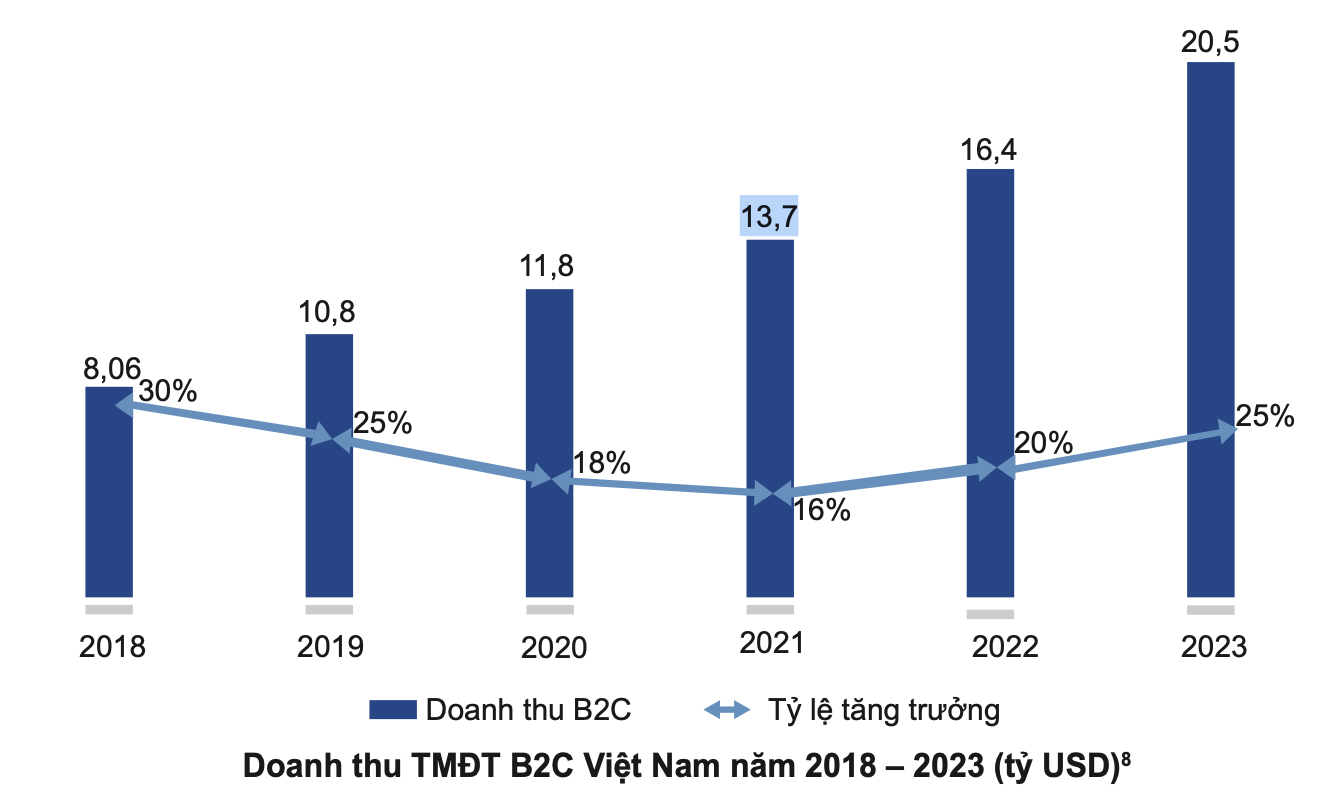
\includegraphics[width=6.5in,height=3.94097in,alt={A graph with numbers and a line AI-generated content may be incorrect.}]{figures/media/image1.png}
\caption[Hình 1: Doanh thu TMĐT B2C Việt Nam năm 2018 -- 2023 (tỷ
USD)]{Hình 1: Doanh thu TMĐT B2C Việt Nam năm 2018 -- 2023 (tỷ
USD)\footnotemark{}}
\end{figure}
\footnotetext{Cục Thương mại điện tử và Kinh tế số - Bộ Công Thương,
  ``Báo cáo Thương mại điện tử Việt Nam 2023'',
  \url{https://valoma.vn/wp-content/uploads/2024/05/BCTMDT2023-file-31-1-pdf.pdf},
  truy cập ngày 25/04/2026.}

\subsubsection{1.2. Giới thiệu về Tập đoàn TH và thương hiệu TH true
MILK}\label{giux1edbi-thiux1ec7u-vux1ec1-tux1eadp-ux111ouxe0n-th-vuxe0-thux1b0ux1a1ng-hiux1ec7u-th-true-milk}

Tập đoàn TH được thành lập vào năm 2009 tại tỉnh Nghệ An, Việt Nam, với
sứ mệnh mang đến nguồn thực phẩm sạch, tươi nguyên, tốt cho sức khỏe và
hoàn toàn từ thiên nhiên cho người tiêu dùng Việt. Tên gọi ``TH'' là
viết tắt của ``True Happiness'' - hạnh phúc thật sự, phản ánh cam kết mà
doanh nghiệp này theo đuổi trong suốt hành trình phát triển của mình.
Sau hơn 15 năm hoạt động, Tập đoàn TH đã trở thành một trong những tập
đoàn kinh tế tư nhân lớn nhất Việt Nam, với tổng vốn đầu tư lên đến hàng
tỷ USD vào nhiều lĩnh vực như chế biến sữa, nông nghiệp công nghệ cao,
dược liệu, tài chính ngân hàng và bất động sản.

Thương hiệu TH True Milk, mảng kinh doanh cốt lõi của tập đoàn, hiện là
đơn vị sở hữu tổng đàn bò sữa lên đến khoảng 70.000 con\footnote{Tập
  đoàn TH, ``Tài liệu giới thiệu và báo cáo định hướng phát triển'',
  \url{https://thgroupglobal.com/storage/attachment/w4LHiea8vHkBcMq5UTJ9RAQmYoJgLbrdjBHVYyOj.pdf},
  truy cập ngày 25/04/2026.}, được chăn nuôi tại các cụm trang trại công
nghệ cao tập trung ở các tỉnh Nghệ An, Đắk Lắk và Đắk Nông. Riêng tại
Đắk Nông, TH đã trở thành nhà đầu tư lớn nhất của tỉnh với tổng vốn đầu
tư lên tới 3,6 tỷ USD\footnote{Báo Nhân Dân, ``Tập đoàn TH đầu tư các dự
  án công nghệ cao trong nông nghiệp và khai khoáng theo định hướng phát
  triển bền vững'',
  \url{https://nhandan.vn/tap-doan-th-dau-tu-cac-du-an-cong-nghe-cao-trong-nong-nghiep-va-khai-khoang-theo-dinh-huong-phat-trien-ben-vung-post805889.html},
  truy cập ngày 25/04/2026.}. Đây là một trong những mô hình nông nghiệp
công nghệ cao quy mô lớn và hiện đại nhất Đông Nam Á, ứng dụng các giải
pháp công nghệ tiên tiến trong toàn bộ quy trình từ chăn nuôi, chế biến
đến phân phối sản phẩm.

Về quy mô thị trường, năm 2024, Tập đoàn TH ghi nhận sự bứt phá trong
phân khúc sữa tươi ở khu vực thành thị, với 51,9\% tổng thị phần, dẫn
đầu cả nước\footnote{Báo Pháp Luật TP.HCM, ``Tập đoàn TH chiếm 51,9\%
  thị phần phân khúc sữa tươi'',
  \url{https://plo.vn/tap-doan-th-chiem-519-thi-phan-phan-khuc-sua-tuoi-post846111.html},
  truy cập ngày 25/04/2026.}, một con số ấn tượng thể hiện vị thế tiên
phong của doanh nghiệp trong cuộc cách mạng sữa tươi sạch. Tính đến cuối
năm 2023, tỷ lệ sữa nước chế biến từ sữa tươi trên toàn thị trường đã
tăng từ chỉ 8\% năm 2008 lên 65,2\%\footnote{Báo Nhân Dân, ``14 dòng sản
  phẩm của Tập đoàn TH đạt Thương hiệu quốc gia 2024'',
  \url{https://nhandan.vn/14-dong-san-pham-cua-tap-doan-th-dat-thuong-hieu-quoc-gia-2024-post843222.html},
  truy cập ngày 25/04/2026.}, minh chứng cho tác động to lớn mà TH đã
tạo ra đối với thói quen tiêu dùng của người Việt.

Với hơn 170 sản phẩm hoàn toàn từ thiên nhiên, TH true MILK không chỉ
dừng lại ở dòng sữa tươi mà còn mở rộng danh mục sang các ngành hàng như
sữa chua ăn, sữa chua uống, sữa hạt, nước uống sữa trái cây, thảo dược
và các sản phẩm dinh dưỡng công thức. Chiến lược đa dạng hóa sản phẩm
này không chỉ giúp TH tiếp cận nhiều phân khúc khách hàng hơn mà còn tạo
ra nhiều cơ hội phát triển trên các kênh thương mại điện tử - nơi người
tiêu dùng ngày càng có xu hướng mua sắm các sản phẩm thực phẩm sức khỏe
trực tuyến.

\subsubsection{1.3. Xu hướng tiêu dùng số và tác động đến ngành hàng
tiêu dùng
nhanh}\label{xu-hux1b0ux1edbng-tiuxeau-duxf9ng-sux1ed1-vuxe0-tuxe1c-ux111ux1ed9ng-ux111ux1ebfn-nguxe0nh-huxe0ng-tiuxeau-duxf9ng-nhanh}

Sự phát triển của thương mại điện tử không chỉ thay đổi kênh mua sắm mà
còn định hình lại toàn bộ hành trình trải nghiệm của người tiêu dùng.
Trong ngành hàng tiêu dùng nhanh, xu hướng mua sắm trực tuyến các mặt
hàng thiết yếu như sữa, thực phẩm và đồ uống đang tăng mạnh, đặc biệt
sau giai đoạn đại dịch Covid-19 đã làm thay đổi thói quen tiêu dùng một
cách đột ngột và bền vững. Người tiêu dùng ngày càng ưu tiên sự tiện
lợi, minh bạch thông tin sản phẩm và cá nhân hóa trải nghiệm mua sắm -
những giá trị mà thương mại điện tử có thể đáp ứng tốt hơn kênh truyền
thống.

Theo báo cáo của AppotaPay về xu hướng thị trường bán lẻ Việt Nam 2025,
mạng lưới cửa hàng bán lẻ truyền thống tuy vẫn chiếm 75\% thị phần với
1,4 triệu cửa hàng tạp hóa và hơn 9.000 chợ\footnote{7}, nhưng tốc độ
tăng trưởng của thương mại điện tử đang nhanh chóng tái định hình thói
quen tiêu dùng. Sự bùng nổ của nền tảng mua sắm trực tuyến với khả năng
cá nhân hóa trải nghiệm và kết hợp mua sắm với giải trí đang thu hút
đông đảo giới trẻ - nhóm khách hàng mục tiêu chủ yếu của TH true MILK.

Ba xu hướng tiêu dùng số nổi bật đang tác động trực tiếp đến chiến lược
thương mại điện tử của các doanh nghiệp FMCG như TH true MILK. Thứ nhất
là xu hướng ``Mua sắm vì sức khỏe'': người tiêu dùng ngày càng tìm kiếm
và ưu tiên các sản phẩm tốt cho sức khỏe, ít đường, ít béo và có nguồn
gốc tự nhiên. Thứ hai là xu hướng ``Ưu tiên sự tiện lợi'': người mua
hàng muốn có trải nghiệm mua sắm nhanh chóng, giao hàng đúng giờ và
thanh toán linh hoạt. Thứ ba là xu hướng ``Yêu cầu minh bạch'': khách
hàng ngày càng quan tâm đến nguồn gốc xuất xứ, quy trình sản xuất và tác
động môi trường của sản phẩm trước khi quyết định mua. Cả ba xu hướng
này đều tương thích hoàn hảo với triết lý kinh doanh và định vị thương
hiệu của TH true MILK.

\subsection*{CHƯƠNG 2: THỰC TRẠNG ÁP DỤNG THƯƠNG MẠI ĐIỆN TỬ VÀ KINH
DOANH SỐ TẠI TH TRUE
MILK}\label{chux1b0ux1a1ng-2-thux1ef1c-trux1ea1ng-uxe1p-dux1ee5ng-thux1b0ux1a1ng-mux1ea1i-ux111iux1ec7n-tux1eed-vuxe0-kinh-doanh-sux1ed1-tux1ea1i-th-true-milk}
\addcontentsline{toc}{subsection}{CHƯƠNG 2: THỰC TRẠNG ÁP DỤNG THƯƠNG MẠI ĐIỆN TỬ VÀ KINH DOANH SỐ TẠI TH TRUE MILK}

\subsubsection{2.1. Chiến lược kinh doanh tổng thể: Định hướng khác biệt
hóa trong môi trường
số}\label{chiux1ebfn-lux1b0ux1ee3c-kinh-doanh-tux1ed5ng-thux1ec3-ux111ux1ecbnh-hux1b0ux1edbng-khuxe1c-biux1ec7t-huxf3a-trong-muxf4i-trux1b0ux1eddng-sux1ed1}

Nền tảng chiến lược của TH true MILK được xây dựng trên nguyên tắc khác
biệt hóa. Thay vì cạnh tranh bằng mức giá thấp hay tập trung vào một
phân khúc hẹp, TH chọn con đường tạo ra sự độc đáo về sản phẩm, dịch vụ
và trải nghiệm khách hàng để biện hộ cho mức giá cao hơn và xây dựng
lòng trung thành thương hiệu bền vững.

Trong bối cảnh kinh doanh số, chiến lược khác biệt hóa của TH true MILK
được thể hiện qua ba trụ cột chính. Trụ cột thứ nhất là ``Chất lượng sản
phẩm vượt trội'': tất cả sản phẩm của TH đều được cam kết là hoàn toàn
từ thiên nhiên, không sử dụng chất bảo quản, không kháng sinh, không
hormone tăng trưởng và đạt các tiêu chuẩn quốc tế nghiêm ngặt. Trụ cột
thứ hai là ``Minh bạch chuỗi cung ứng'', TH sở hữu mô hình khép kín từ
trang trại đến kệ hàng, cho phép kiểm soát và truy xuất nguồn gốc toàn
bộ quy trình sản xuất. Trụ cột thứ ba là ``Đổi mới liên tục'': TH không
ngừng nghiên cứu và tung ra các sản phẩm mới đón đầu xu hướng tiêu dùng
sức khỏe.

Trong môi trường số, chiến lược khác biệt hóa này được khuếch đại và
truyền tải hiệu quả hơn nhờ các công cụ thương mại điện tử và tiếp thị
kỹ thuật số. Khái niệm ``mật độ thông tin'' trong lý thuyết thương mại
điện tử cho phép TH cung cấp cho người tiêu dùng lượng thông tin đầy đủ,
minh bạch và cập nhật về quy trình chăn nuôi hữu cơ, tiêu chuẩn chất
lượng và giá trị dinh dưỡng của từng sản phẩm, điều mà kênh bán lẻ
truyền thống không thể thực hiện với cùng chi phí và quy mô. Đây chính
là lợi thế cạnh tranh số mà TH đã và đang khai thác triệt để.

\begin{figure}
\centering
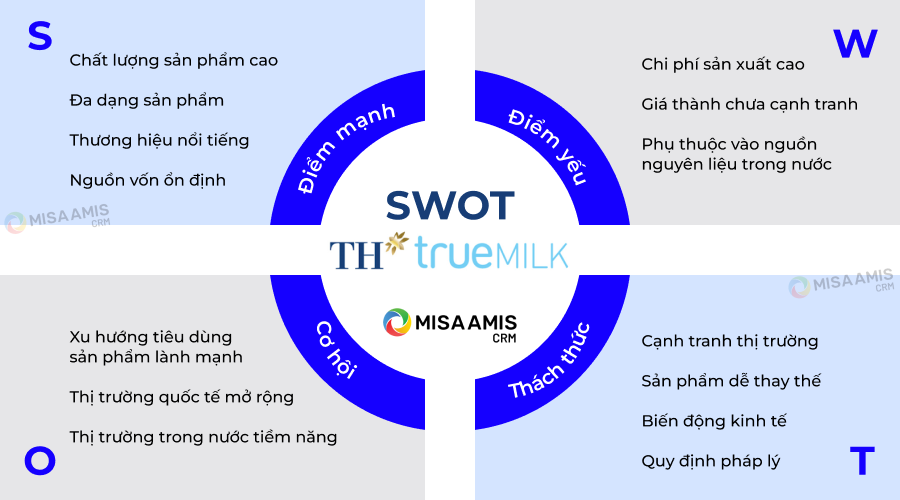
\includegraphics[width=6.5in,height=3.61111in,alt={A diagram of a milk company AI-generated content may be incorrect.}]{figures/media/image2.png}
\caption[Hình 2: Mô hình SWOT của TH True Milk góp vai trò lớn trong
chiến lược kinh doanh của thương hiệu]{Hình 2: Mô hình SWOT của TH True
Milk góp vai trò lớn trong chiến lược kinh doanh của thương
hiệu\footnotemark{}}
\end{figure}
\footnotetext{MISA AMIS, ``Chiến lược kinh doanh của TH True Milk'',
  \url{https://amis.misa.vn/30576/chien-luoc-kinh-doanh-cua-th-true-milk/},
  truy cập ngày 25/04/2026.}

Theo phân tích mô hình SWOT, điểm mạnh cốt lõi của TH true MILK trong
môi trường số nằm ở ba yếu tố: Một là thương hiệu được xây dựng và củng
cố qua nhiều năm với mức độ nhận diện cao trong phân khúc sức khỏe; hai
là khả năng tích hợp công nghệ cao vào toàn bộ chuỗi giá trị, tạo ra lợi
thế cạnh tranh khó bị sao chép; ba là hệ thống phân phối đa kênh rộng
khắp, kết hợp giữa cửa hàng vật lý TH true mart, sàn thương mại điện tử
và kênh giao hàng nhanh. Ba yếu tố này tạo nên một ``bộ giáp'' cạnh
tranh vững chắc trong kỷ nguyên kinh doanh số.

\subsubsection{2.2. Mô hình Thương mại điện tử B2C và D2C của TH true
MILK}\label{muxf4-huxecnh-thux1b0ux1a1ng-mux1ea1i-ux111iux1ec7n-tux1eed-b2c-vuxe0-d2c-cux1ee7a-th-true-milk}

TH true MILK hoạt động chủ yếu theo mô hình B2C - mô hình kinh doanh
trực tiếp giữa doanh nghiệp và người tiêu dùng cuối. Trong những năm gần
đây, TH đã tiến thêm một bước quan trọng khi chuyển dịch sang mô hình
D2C, nghĩa là nhà sản xuất phân phối trực tiếp đến tay người tiêu dùng
mà không cần qua trung gian. Đây là một chiến lược đột phá trong ngành
FMCG, nơi các trung gian phân phối truyền thống từ lâu đã chi phối chuỗi
giá trị.

Mô hình D2C của TH true MILK được triển khai thông qua hai kênh chính.
Kênh thứ nhất là hệ thống cửa hàng TH true mart - chuỗi cửa hàng bán lẻ
do TH trực tiếp sở hữu và vận hành, trải rộng trên khắp cả nước. Đây là
kênh vật lý trong mô hình D2C, nơi người tiêu dùng có thể trực tiếp trải
nghiệm sản phẩm TH trong một không gian thương hiệu được thiết kế đồng
bộ và nhất quán. Kênh thứ hai là website bán hàng trực tuyến và ứng dụng
di động, cho phép khách hàng đặt hàng và nhận sản phẩm ngay tại nhà.

Ưu điểm vượt trội của mô hình D2C trong thương mại điện tử là khả năng
kiểm soát hoàn toàn trải nghiệm khách hàng từ đầu đến cuối. Khi bán hàng
qua các kênh trung gian như siêu thị hay nhà phân phối, TH mất đi cơ hội
tiếp xúc trực tiếp với người tiêu dùng và xây dựng mối quan hệ cá nhân
hóa. Ngược lại, kênh D2C cho phép TH thu thập dữ liệu khách hàng quý
giá, hiểu rõ hành vi mua sắm, sở thích cá nhân và phản hồi về sản phẩm
để từ đó liên tục cải thiện cả sản phẩm lẫn trải nghiệm mua sắm.

Ngoài ra, mô hình D2C cũng mang lại lợi thế về biên độ lợi nhuận khi TH
có thể loại bỏ hoặc giảm bớt các chi phí hoa hồng cho trung gian phân
phối, từ đó có thêm nguồn lực để đầu tư vào chất lượng sản phẩm và cung
cấp giá trị tốt hơn cho khách hàng, đồng thời xây dựng được tệp khách
hàng trung thành mạnh hơn nhờ mối quan hệ trực tiếp và cá nhân hóa.

Bên cạnh kênh D2C, TH true MILK còn duy trì sự hiện diện mạnh mẽ trên
các sàn thương mại điện tử B2C lớn như Shopee, Lazada, TikTok Shop và
các nền tảng giao đồ ăn như ShopeeFood và GrabMart. Chiến lược kết hợp
D2C và B2C đa kênh này cho phép TH tiếp cận đa dạng tệp khách hàng trong
khi vẫn duy trì sự kiểm soát thương hiệu và chất lượng dịch vụ.

\subsubsection{\texorpdfstring{2.3. Tích hợp công nghệ trong chuỗi giá
trị
}{2.3. Tích hợp công nghệ trong chuỗi giá trị }}\label{tuxedch-hux1ee3p-cuxf4ng-nghux1ec7-trong-chuux1ed7i-giuxe1-trux1ecb}

Một trong những điểm khác biệt nổi bật nhất của TH true MILK so với các
đối thủ cạnh tranh trong ngành sữa là mức độ tích hợp công nghệ số vào
toàn bộ chuỗi giá trị: từ khâu chăn nuôi và thu mua sữa nguyên liệu, cho
đến chế biến, bảo quản, vận chuyển và phân phối đến tay người tiêu dùng.
Đây chính là bản chất của kinh doanh số: không chỉ đơn thuần là việc bán
hàng trực tuyến mà còn là việc số hóa toàn diện các quy trình nội bộ để
tạo ra hiệu quả vận hành vượt trội và chất lượng sản phẩm đồng nhất.

Tại các trang trại bò sữa, TH ứng dụng công nghệ nông nghiệp chính xác
và hệ thống quản lý trang trại thông minh. Mỗi con bò được gắn chip theo
dõi sức khỏe và năng suất sữa theo thời gian thực, cho phép đội ngũ kỹ
thuật viên giám sát và phản ứng kịp thời với mọi biến động. Hệ thống tự
động hóa vắt sữa với các robot vắt sữa hiện đại đảm bảo vệ sinh và nhất
quán trong quy trình thu hoạch. Dữ liệu từ tất cả các khâu này được tích
hợp vào nền tảng quản lý trung tâm, cho phép lãnh đạo doanh nghiệp theo
dõi hiệu quả vận hành và đưa ra quyết định dựa trên dữ liệu.

Trong khâu chế biến và sản xuất, nhà máy TH tại Nghệ An áp dụng hệ thống
tự động hóa và trí tuệ nhân tạo để kiểm soát chất lượng sản phẩm theo
thời gian thực. Các cảm biến và hệ thống Mạng lưới vạn vật kết nối
Internet được triển khai xuyên suốt dây chuyền sản xuất để phát hiện và
loại bỏ ngay các lô sản phẩm không đạt tiêu chuẩn. Hệ thống ứng dụng
phần mềm đa phân hệ (ERP) kết nối toàn bộ các bộ phận từ sản xuất, kho
bãi, hậu cần đến tài chính và bán hàng, đảm bảo thông tin được đồng bộ
và cập nhật liên tục.

Đặc biệt quan trọng đối với chiến lược thương mại điện tử là hệ thống
truy xuất nguồn gốc số mà TH đã triển khai. Mỗi sản phẩm TH true MILK
được gắn mã QR cho phép người tiêu dùng tra cứu toàn bộ hành trình của
sản phẩm: từ trang trại nào sữa được vắt, thời gian thu hoạch, quy trình
chế biến, nhiệt độ bảo quản cho đến hạn sử dụng. Tính năng ``phổ biến''
của công nghệ thương mại điện tử cho phép người tiêu dùng thực hiện việc
tra cứu này bất kỳ lúc nào, bất kỳ ở đâu chỉ với chiếc điện thoại thông
minh, củng cố mạnh mẽ thông điệp ``Thật sự thiên nhiên'' của thương
hiệu.

Về hệ thống chuỗi cung ứng và phân phối số, TH đã đầu tư đáng kể vào hạ
tầng chuỗi lạnh để đảm bảo chất lượng sản phẩm tươi trong suốt quá trình
vận chuyển từ nhà máy đến tay người tiêu dùng. Hệ thống quản lý đơn hàng
trực tuyến tích hợp với các nền tảng thương mại điện tử và ứng dụng giao
hàng cho phép TH xử lý đơn hàng tự động, tối ưu hóa tuyến đường giao
hàng và cung cấp thông tin giao hàng thời gian thực cho khách hàng.

\subsubsection{2.4. Chiến lược đa kênh và hoạt động trên các sàn thương
mại điện
tử}\label{chiux1ebfn-lux1b0ux1ee3c-ux111a-kuxeanh-vuxe0-houx1ea1t-ux111ux1ed9ng-truxean-cuxe1c-suxe0n-thux1b0ux1a1ng-mux1ea1i-ux111iux1ec7n-tux1eed}

TH true MILK đã triển khai chiến lược phân phối và tiếp cận khách hàng
đồng bộ và liền mạch trên tất cả các kênh bán hàng như một trụ cột cốt
lõi trong chiến lược thương mại điện tử. Thay vì coi các kênh bán hàng
là độc lập và riêng biệt, TH xây dựng hệ sinh thái bán hàng tích hợp,
nơi khách hàng có thể bắt đầu hành trình mua sắm ở bất kỳ kênh nào và
chuyển sang kênh khác một cách mượt mà mà không mất đi trải nghiệm liên
tục.

Hệ thống phân phối của TH hiện bao gồm: Một là mạng lưới cửa hàng TH
true mart trên toàn quốc đóng vai trò là kênh vật lý trực tiếp; hai là
website thương mại điện tử tại thmilk.vn là kênh số do TH sở hữu; ba là
gian hàng chính thức trên các sàn thương mại điện tử lớn bao gồm Shopee
Mall, Lazada, TikTok Shop; bốn là TH true mart trên ứng dụng giao đồ ăn
ShopeeFood và GrabMart; năm là kênh phân phối truyền thống qua siêu thị,
đại lý và điểm bán lẻ trên cả nước. Sự kết hợp đồng bộ giữa tất cả các
kênh này tạo ra một mạng lưới phân phối phủ sóng rộng khắp và linh hoạt,
đảm bảo TH true MILK có mặt ở mọi nơi khách hàng cần mua sắm.

\begin{figure}
\centering
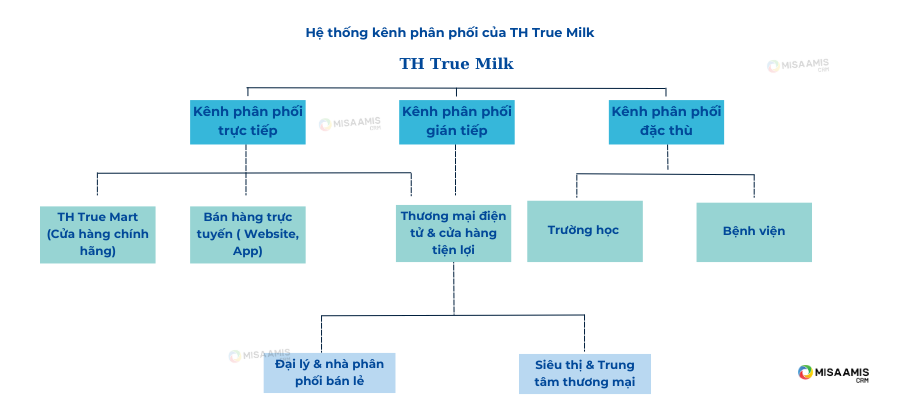
\includegraphics[width=6.5in,height=2.88889in,alt={A diagram of milk with blue and green rectangles AI-generated content may be incorrect.}]{figures/media/image3.png}
\caption[Hình 3: Hệ thống kênh phân phối của TH true MILK]{Hình 3: Hệ
thống kênh phân phối của TH true MILK\footnotemark{}}
\end{figure}
\footnotetext{MISA AMIS, ``Hệ thống phân phối của TH True Milk'',
  \url{https://amis.misa.vn/165501/he-thong-phan-phoi-cua-th-true-milk/},
  truy cập ngày 25/04/2026.}

Trên nền tảng Shopee, TH true MILK đã xây dựng chiến lược nội dung,
chính sách giá, chương trình khuyến mãi và quản lý vận hành gian hàng
trực tuyến một cách chuyên nghiệp và bài bản.

Trên TikTok Shop - nền tảng thương mại điện tử đang phát triển nhanh
nhất tại Việt Nam, TH true MILK tích cực khai thác hình thức livestream
bán hàng và sản xuất nội dung video ngắn thu hút, chuyển đổi người xem
thành người mua một cách hiệu quả. Theo các báo cáo thị trường, tỷ lệ
chuyển đổi từ xem livestream đến mua hàng trong ngành thực phẩm và đồ
uống tại TikTok Shop đã tăng mạnh, đặc biệt khi thương hiệu kết hợp yếu
tố giải trí và giáo dục dinh dưỡng trong nội dung.

\subsubsection{2.5. Ứng dụng tiếp thị số và quản lý dữ liệu khách
hàng}\label{ux1ee9ng-dux1ee5ng-tiux1ebfp-thux1ecb-sux1ed1-vuxe0-quux1ea3n-luxfd-dux1eef-liux1ec7u-khuxe1ch-huxe0ng}

Tiếp thị số là một trong những công cụ quan trọng nhất mà TH true MILK
đang tận dụng để xây dựng và duy trì vị thế thương hiệu trong môi trường
số cạnh tranh khốc liệt. Chiến lược tiếp thị số của TH được xây dựng
trên nền tảng tích hợp nhiều kênh và công cụ, từ SEO/SEM (tìm kiếm tự
nhiên và có trả phí), mạng xã hội như Facebook, Instagram, TikTok,
YouTube; tiếp thị email cho đến tiếp thị dựa trên người có ảnh hưởng và
tiếp thị dựa trên hiệu suất.

Trong lĩnh vực tiếp thị qua mạng xã hội, TH true MILK duy trì sự hiện
diện tích cực trên tất cả các nền tảng mạng xã hội lớn với chiến lược
nội dung nhất quán và phong phú. Nội dung do người dùng tạo ra được
khuyến khích và khuếch đại thông qua các chiến dịch hashtag và thách
thức trực tuyến. Đặc biệt, TH khai thác triệt để xu hướng ``Nội dung Sức
khỏe và Sống khỏe'' bao gồm các video và bài đăng chia sẻ kiến thức dinh
dưỡng, công thức nấu ăn lành mạnh và câu chuyện về quy trình sản xuất
sữa hữu cơ, nhằm xây dựng hình ảnh ``Chuyên gia dinh dưỡng'' cho thương
hiệu trong tâm trí người tiêu dùng.

Về quản lý dữ liệu khách hàng, TH đã đầu tư vào hệ thống quản lý tích
hợp để thu thập, phân tích và khai thác dữ liệu từ nhiều điểm chạm khách
hàng khác nhau: từ website, ứng dụng di động, kênh mạng xã hội đến cửa
hàng vật lý. Dữ liệu này cho phép TH phân khúc khách hàng một cách chi
tiết và thực hiện các chiến dịch marketing cá nhân hóa, gửi đúng thông
điệp đến đúng người vào đúng thời điểm. Theo các nghiên cứu về hiệu quả
marketing số, các chiến dịch tiếp thị qua email cá nhân hóa có tỷ lệ mở
cao hơn 26\% và tỷ lệ chuyển đổi cao hơn 6 lần so với các chiến dịch đại
trà.

TH true MILK cũng ứng dụng công nghệ dữ liệu lớn và trí tuệ nhân tạo vào
phân tích xu hướng tiêu dùng và dự báo nhu cầu. Bằng cách phân tích dữ
liệu hành vi mua sắm từ các kênh thương mại điện tử, TH có thể dự báo
chính xác hơn nhu cầu sản phẩm theo từng địa lý, mùa vụ và phân khúc
khách hàng, từ đó tối ưu hóa kế hoạch sản xuất và quản lý tồn kho, giảm
thiểu lãng phí và đảm bảo sản phẩm tươi luôn sẵn có.

Chiến lược tiếp thị nội dung của TH tập trung vào việc truyền tải câu
chuyện thương hiệu một cách chân thực và có chiều sâu. Các nội dung về
hành trình từ trang trại hữu cơ đến sản phẩm sữa tươi sạch, về cam kết
bảo vệ môi trường và trách nhiệm xã hội của doanh nghiệp được sản xuất
và phân phối liên tục qua các kênh số. Hình thức này không chỉ thu hút
và giữ chân người tiêu dùng mà còn xây dựng niềm tin thương hiệu yếu tố
quyết định đặc biệt quan trọng đối với ngành thực phẩm và sức khỏe.

\subsubsection{2.6. Kết quả kinh doanh số và thành tích nổi bật trên nền
tảng thương mại điện
tử}\label{kux1ebft-quux1ea3-kinh-doanh-sux1ed1-vuxe0-thuxe0nh-tuxedch-nux1ed5i-bux1eadt-truxean-nux1ec1n-tux1ea3ng-thux1b0ux1a1ng-mux1ea1i-ux111iux1ec7n-tux1eed}

Những nỗ lực đầu tư và triển khai chiến lược thương mại điện tử một cách
bài bản đã mang lại cho TH true MILK những thành quả kinh doanh số ấn
tượng và có thể đo lường được. Năm 2023 là một năm đặc biệt thành công
đối với TH trong lĩnh vực thương mại điện tử: doanh thu từ các kênh
thương mại điện tử tăng trưởng 45\% so với năm 2022\footnote{Báo Sài Gòn
  Giải Phóng, ``TH true MILK năm 2023: Những dấu ấn nổi bật trong hành
  trình phụng sự vì sức khỏe cộng đồng'',
  \url{https://www.sggp.org.vn/th-true-milk-nam-2023-nhung-dau-an-noi-bat-trong-hanh-trinh-phung-su-vi-suc-khoe-cong-dong-post726030.html},
  truy cập ngày 25/04/2026.}, một con số vượt xa tốc độ tăng trưởng
chung của thị trường thương mại điện tử Việt Nam. Thành tích này được
ghi nhận đồng đều trên nhiều nền tảng và kênh bán hàng số khác nhau.

Cụ thể, trên sàn TikTok Shop, TH true MILK đạt vị trí Top 1 doanh thu
ngành hàng sữa và sản phẩm từ sữa\footnote{Tạp chí Kinh tế Sài Gòn, ``TH
  true mart chiến thắng hạng mục Thương hiệu cung ứng hàng hóa phong phú
  trên sàn thương mại điện tử'',
  \url{https://thesaigontimes.vn/th-true-mart-chien-thang-hang-muc-thuong-hieu-cung-ung-hang-hoa-phong-phu-tren-san-thuong-mai-dien-tu-hang-dau-viet-nam/},
  truy cập ngày 25/04/2026.}, một thành tích đặc biệt ý nghĩa trên nền
tảng mua sắm kết hợp giải trí đang thu hút hàng chục triệu người dùng
mỗi tháng. Trên sàn Shopee, TH liên tục nằm trong Top 3 doanh thu ngành
hàng trong tất cả các chiến dịch mega sale lớn\footnote{17} của năm cho
thấy sự ổn định và hiệu quả trong vận hành gian hàng thương mại điện tử.
Trên nền tảng ShopeeFood, TH true mart tiếp tục khẳng định vị thế thương
hiệu FMCG hàng đầu với đánh giá 5 sao từ người dùng về chất lượng sản
phẩm, tốc độ giao hàng và chương trình khuyến mãi. Đây là minh chứng cho
sự đánh giá cao của thị trường đối với chiến lược phân phối đa kênh và
chất lượng dịch vụ của TH trong hệ sinh thái thương mại điện tử.

Về tăng trưởng sản phẩm cụ thể, năm 2023 ghi nhận: ngành hàng nước uống
sữa trái cây TH true JUICE MILK đạt mức tăng 62\%; ngành hàng sữa chua
ăn tăng 10,3\%, gấp đôi mức tăng dự báo chung của ngành\footnote{16}.
Tập đoàn TH nói chung đạt mức tăng trưởng doanh thu hai con số, cao gấp
nhiều lần mức tăng trưởng chung của ngành hàng tại khu vực thành thị.
Những con số này phản ánh hiệu quả của chiến lược kết hợp giữa đổi mới
sản phẩm và đầu tư vào kênh thương mại điện tử.

Về xếp hạng thương hiệu, Theo báo cáo Dấu ấn Thương hiệu Việt Nam 2023
được thực hiện hàng năm bởi tổ chức hàng đầu thế giới về dữ liệu, nghiên
cứu và tư vấn - Kantar Worldpanel Việt Nam, TH true MILK tiếp tục giữ
vững vị trí trong ``Top những thương hiệu sữa và sản phẩm từ sữa được
lựa chọn nhiều nhất'', đây là năm thứ ba liên tiếp TH đạt được danh hiệu
này\footnote{Báo Dân Trí, ``Thương mại điện tử sẽ tiếp tục bứt phá'',
  \url{https://dansinh.dantri.com.vn/tien-luong-tien-cong/thuong-mai-dien-tu-se-tiep-tuc-but-pha-20250213163955355.htm},
  truy cập ngày 25/04/2026.}. Kantar ghi nhận TH là thương hiệu tăng
trưởng rất nhanh, không chỉ trong thị trường sữa, với sự phát triển mạnh
mẽ của các sản phẩm ít đường và không đường, phù hợp với xu hướng tiêu
dùng sức khỏe đang ngày càng lan rộng.

\input{chapters_3_5.tex}

\section*{TÀI LIỆU THAM KHẢO}
\addcontentsline{toc}{section}{TÀI LIỆU THAM KHẢO}

\begin{thebibliography}{99}
\bibitem{vecom2025} Hiệp hội Thương mại điện tử Việt Nam (VECOM). Báo cáo Chỉ số Thương mại điện tử Việt Nam 2025. \url{https://vecom.vn/bao-cao-chi-so-thuong-mai-dien-tu-viet-nam-2025}.
\bibitem{metric2024} Metric. Báo cáo toàn cảnh thị trường sàn bán lẻ trực tuyến 2024.
\bibitem{cuctmdt2023} Cục Thương mại điện tử và Kinh tế số -- Bộ Công Thương. Báo cáo Thương mại điện tử Việt Nam 2023. \url{https://valoma.vn/wp-content/uploads/2024/05/BCTMDT2023-file-31-1-pdf.pdf}.
\bibitem{appotapay2025} AppotaPay. Báo cáo xu hướng thị trường bán lẻ Việt Nam 2025.
\bibitem{vneconomy2024} VnEconomy. ``Thương mại điện tử Việt Nam tiếp tục bứt phá, hướng đến mục tiêu 25 tỷ USD vào 2025''. \url{https://vneconomy.vn/thuong-mai-dien-tu-viet-nam-tiep-tuc-but-pha-huong-den-muc-tieu-25-ty-usd-vao-2025.htm}.
\bibitem{thgroup2026} Tập đoàn TH. Tài liệu giới thiệu và báo cáo định hướng phát triển. \url{https://thgroupglobal.com/storage/attachment/w4LHiea8vHkBcMq5UTJ9RAQmYoJgLbrdjBHVYyOj.pdf}.
\bibitem{nhandanth2026} Báo Nhân Dân. ``Tập đoàn TH đầu tư các dự án công nghệ cao trong nông nghiệp và khai khoáng theo định hướng phát triển bền vững''. \url{https://nhandan.vn/tap-doan-th-dau-tu-cac-du-an-cong-nghe-cao-trong-nong-nghiep-va-khai-khoang-theo-dinh-huong-phat-trien-ben-vung-post805889.html}.
\bibitem{ploth2026} Báo Pháp Luật TP.HCM. ``Tập đoàn TH chiếm 51,9\% thị phần phân khúc sữa tươi''. \url{https://plo.vn/tap-doan-th-chiem-519-thi-phan-phan-khuc-sua-tuoi-post846111.html}.
\bibitem{nhandan2024product} Báo Nhân Dân. ``14 dòng sản phẩm của Tập đoàn TH đạt Thương hiệu quốc gia 2024''. \url{https://nhandan.vn/14-dong-san-pham-cua-tap-doan-th-dat-thuong-hieu-quoc-gia-2024-post843222.html}.
\bibitem{sggp2026} Báo Sài Gòn Giải Phóng. ``TH true MILK năm 2023: Những dấu ấn nổi bật trong hành trình phụng sự vì sức khỏe cộng đồng''. \url{https://www.sggp.org.vn/th-true-milk-nam-2023-nhung-dau-an-noi-bat-trong-hanh-trinh-phung-su-vi-suc-khoe-cong-dong-post726030.html}.
\bibitem{ktsaigon2026} Tạp chí Kinh tế Sài Gòn. ``TH true mart chiến thắng hạng mục Thương hiệu cung ứng hàng hóa phong phú trên sàn thương mại điện tử''. \url{https://thesaigontimes.vn/th-true-mart-chien-thang-hang-muc-thuong-hieu-cung-ung-hang-hoa-phong-phu-tren-san-thuong-mai-dien-tu-hang-dau-viet-nam/}.
\bibitem{dantri2026} Báo Dân Trí. ``Thương mại điện tử sẽ tiếp tục bứt phá''. \url{https://dansinh.dantri.com.vn/tien-luong-tien-cong/thuong-mai-dien-tu-se-tiep-tuc-but-pha-20250213163955355.htm}.
\bibitem{thmilkhome} TH true MILK, website chính thức. Truy cập từ \url{https://thtruemilk.com.vn}.
\bibitem{thtruemartdelivery} TH true MILK, Dịch vụ giao hàng tận nhà. Truy cập từ \url{https://thtruemilk.com.vn/dich-vu-giao-hang}.
\bibitem{vinamilkterms} Vinamilk, Điều khoản sử dụng Vinamilk Shop. Truy cập từ \url{https://vinamilkshop.vn}.
\bibitem{fresh2024} Fresh Milk Co., Ltd. (Thái Lan). Báo cáo hoạt động TMĐT năm 2024. Bangkok.
\bibitem{organickorea2024} Korea Organic Association. Xu hướng bán hàng hữu cơ trực tuyến tại Hàn Quốc. Seoul, 2024.
\bibitem{iresearch2024} iRESEARCH. Southeast Asia E-commerce Market Report 2024. Singapore: iRESEARCH Pte. Ltd.
\bibitem{statista2024} Statista. E-commerce Sales in Vietnam 2020--2024. Truy cập từ \url{https://www.statista.com}.
\end{thebibliography}

% --- End inserted content ---

\end{document}

